\subsubsection{Temperatursensor}\label{sec:Temperatursensor}
In der Testkammer befinden sich zwei Temperatursensoren mit integriertem Feuchtigkeitssensoren. Diese messen die Temperatur sowie die Feuchtigkeit in der Kammer. Dadurch können die Sensorwerte der Kammer und des CubeSat verglichen werden.\\
\vspace{3mm}
Für diese Anwendung wird der Temperatursensor \textbf{AM2302} \autocite{AM2302} verwendet. Der Anschluss an den \raspi erfolgt durch die PCB. Der Sensor wird mit 3 Pins an die PCB angeschlossen.\\
\vspace{3mm}
\begin{table}[H]
    \centering
    \begin{tabular}{ | c | c | } 
  \hline
   VDD & 5 Volt\\ 
  \hline
   GND & Ground\\ 
  \hline
   Data & GPIO7 und GPIO8\\ 
  \hline
\end{tabular}
    \caption{Pinbelegung Temperatursensor}
\end{table}
Um beide Sensoren in der Testkammer zu montieren, wurde ein Gehäuse in SolidWorks entworfen. Danach wurden die Teile mit dem 3D-Drucker ausgedruckt.\\
\vspace{2mm}
\begin{figure}[H]
\centering
\includegraphics[scale=0.6]{image/Gehäusetemp.png}
\caption{Gehäuse Temperatursensor}
\end{figure}
\newpage
Um den Temperatursensor zu verwenden, wird eine Bibliothek benötigt. Die Bibliothek wird von Adafruit bereitgestellt. Um diese zu installieren wird folgender Befehl auf dem \raspi ausgeführt:\\
\begin{verbatim}
pip3 install adafruit-circuitpython-dht
\end{verbatim}
Durch die Bibliothek\autocite{Adafruit_DHT} wird das Auslesen des Sensors vereinfacht. Mit wenigen Befehlen kann der Sensor die Temperatur und die Feuchtigkeit messen.\\
\vspace{3mm}
\begin{figure}[H]
    \centering
    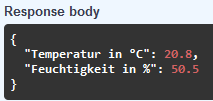
\includegraphics[scale=1.5]{image/Tempausgabe.png}
    \caption{Temperatursensorausgabe}
    \label{fig:enter-label}
\end{figure}
Die Messung mit dem Temperatursensor wurden in einem normalen Zimmer mit Raumtemperatur durchgeführt. Die ermittelten Daten für Temperatur und Feuchtigkeit werden in der oberen Abbildung abgebildet.\\
\vspace{3mm}
Die Programmierung für das Testprogramm befindet sich im Kapitel \ref{sec:Testprogramm Temp}, und der Programm Abschnitt für die API im Kapitel \ref{sec:API-Temp}




